\section{Photometric Redshifts}\label{sec:pz}

A one page summary of our analysis of the {\tt OpSim} and {\tt ALTSched} results is provided in Section \ref{mlg_sec:pz_summary}. A more in-depth evaluation of how the photometric redshifts derived from LSST photometry will evolve over the 10 year survey, for a variety of observing strategies that includes the formal {\tt OpSim} runs along with more general scenarios in which e.g., 5\% of the total observing time is redistributed to or from each filter in turn, is currently underway and being documented in this Overleaf draft: \url{https://www.overleaf.com/read/fgnvddbnrmgk}.


% % % % % % % % % % % % % % % % % % % % % % % % % % % % %
\subsection{Evaluating the Photometric Evolution of the Observing Strategies}\label{ssec:pz_opsim_phot}

To evaluate the photometric quality produced by each of the proposed observing strategies, we use the Metric Analysis Framework (MAF) as follows.

{\bf Slicer:} We use a HEALpix slicer with {\tt nside} $=16$ and a random dither to the field RA and Dec ({\tt latCol = randomDitherFieldPerNightRa} and {\tt lonCol = randomDitherFieldPerNightDec}). This slicer returns metrics in fields with an approximate resolution of $220$ arcminutes ($3.67$ degrees), similar to a single LSST pointing, and the dither helps to smooth out field-to-field variations in a realistic way. The dither option is not needed or applied with simulations from the feature-based scheduler ({\tt rolling\_10yrs}) or {\tt ALTSched}. 

{\bf Metric:} We use {\tt ExgalM5}, which returns the $5{\sigma}$ limiting magnitude for a given filter, corrected for Galactic dust extinction. We require that a given field have observations in all $6$ filters to be considered as conceivably be appropriate for photo-$z$ estimation (and recall that we impose the constraint that a galaxy must be {\it detected} in $griz$ to get a photo-$z$ estimate). We furthermore impose that the Galactic extinction $E(B-V) \leq 0.2$ mag and that the $5{\sigma}$ $i$-band detection limit be at least $24.5/25.0/25.5/26.0$ magnitudes at $1/3/6/10$ years.

{\bf Bundle:} We run the metric and slicer for years $1$, $3$, $6$, and $10$. We only consider images that are obtained as part of the WFD survey component, to avoid depth pockets from mini-surveys or deep drilling fields. We furthermore only consider fields with a Galactic longitude of $60 < l < 300$ degrees {\em or} Galactic latitude of $b>30$ degrees, as would a cosmological science analysis relying on the LSST photo-$z$, but the $E(B-V) \leq 0.2$ mag is actually more constraining than this location constraint.

Using the above slicer, metric, and bundle, we generate a single file per year per {\tt OpSim} or {\tt ALTSched} run, in which each row represents a ``field" that was observed in all $6$ filters as part of the WFD survey, and the columns are right ascension, declination, and the $5{\sigma}$ limiting magnitude in filters $ugrizy$. 

In Figures \ref{fig:maglims} and \ref{fig:maglims_2} we plot the evolution in the median limiting magnitude for each filter (individual plots), as a function of survey year, for the observing strategy simulations discussed in Section \ref{sec:intro}. Figure \ref{fig:maglims} compares {\tt OpSim} runs that change the WFD survey area and/or the visit strategy, while Figure \ref{fig:maglims_2} investigates the impact of adopting a rolling cadence. Additionally, the bottom panel of Figure \ref{fig:maglims_2} compares the baseline runs of {\tt OpSim} and {\tt ALTSched}. As we can see from Figures \ref{fig:maglims} and \ref{fig:maglims_2}, many of the runs produce a photometric evolution that is equivalent to the baseline, {\tt kraken\_2026}, which is always plotted with dark blue circles. 

{\bf Figure \ref{fig:maglims}, top panel --} For runs that change the survey area, it is clear that including the Galactic Plane as part of a $18,000$ square degree WFD survey area ({\tt colossus\_2664}, red triangles) does not appreciably degrade the photometric results. However, extending the survey area at the expense of depth does make a significant impact, whether or not the same-night revisits are executed ({\tt pontus\_2002}, green squares, and {\tt kraken\_2044}, yellow triangles). It appears that the impact to the overall depth is slightly worse if the revisits are done, and so we will only simulate photo-$z$ results for the large WFD option ({\tt pontus\_2002}). 

{\bf Figure \ref{fig:maglims}, bottom panel --} For runs that change the survey's visits, we can see that avoiding revisits ({\tt colossus\_2667}) or snaps ({\tt kraken\_2042}) does not have a significant impact on the median depth evolution, and so we will only simulate photo-$z$ for the ``many visits" option with 20/40 second exposures in filters $grizy$/$u$ ({\tt pontus\_2489}). 

{\bf Figure \ref{fig:maglims_2}, top panel --} For runs that adopt a rolling cadence for the baseline WFD area of $18,000$ square degrees, the effect on the photometric quality is significant: a rolling cadence ({\tt rolling\_10yrs}, magenta pentagons) produces a degraded median depth in nearly all filters at all times including year 10 (compared to the baseline, blue circles). Exactly why this is the case, and why the issue is exacerbated for $y$-band, is unclear at this time -- but may be because {\tt rolling\_10yrs} was pretty good about only taking $y$-band when the full moon was up (i.e., not spending dark time on $y$-band visits)\footnote{From a conversation with Peter Yoachim.}. For this work, we will only simulate photo-$z$ for the option with two declination bands and a 25\% WFD component in a baseline area of $18,000$ square degrees ({\tt rolling\_10yrs}). We do not evaluate the {\tt OpSim} runs that adopt a rolling cadence over the wider PanSTARRs-like $25,000$ square degrees, {\tt mothra\_2049} and {\tt nexus\_2097}, because they suffer from the same bug of missing visits as {\tt pontus\_2502} and {\tt mothra\_2045}.

{\bf Figure \ref{fig:maglims_2}, bottom panel --} We also show the photometric evolution of the {\tt ALTSched} simulations without and with a rolling cadence that alternates between two declination bands (cyan circles and black pentagons, respectively). These differ enough from the {\tt OpSim} baseline run enough that we will simulate photo-$z$ results for both {\tt ALTSched} observing strategies. In particular, the improved depth in all filters with {\tt ALTSched}'s rolling cadence is significant (black pentagons at x-axis year = 1). This is attributed to the fact that the {\tt ALTSched} rolling cadence only observes one declination band in year 1, where as {\tt OpSim}'s {\tt rolling\_10yrs} allows the deprioritized declination band $25\%$ of the baseline number of visits. Furthermore, by year 10 the rolling and non-rolling versions of {\tt ALTSched} have converged at a common final depth in all filters, unlike the {\tt OpSim}'s baseline and rolling cadence (in which the rolling cadence achieves a shallower final result; the underlying cause of this is unclear).

\begin{figure*}
\begin{center}
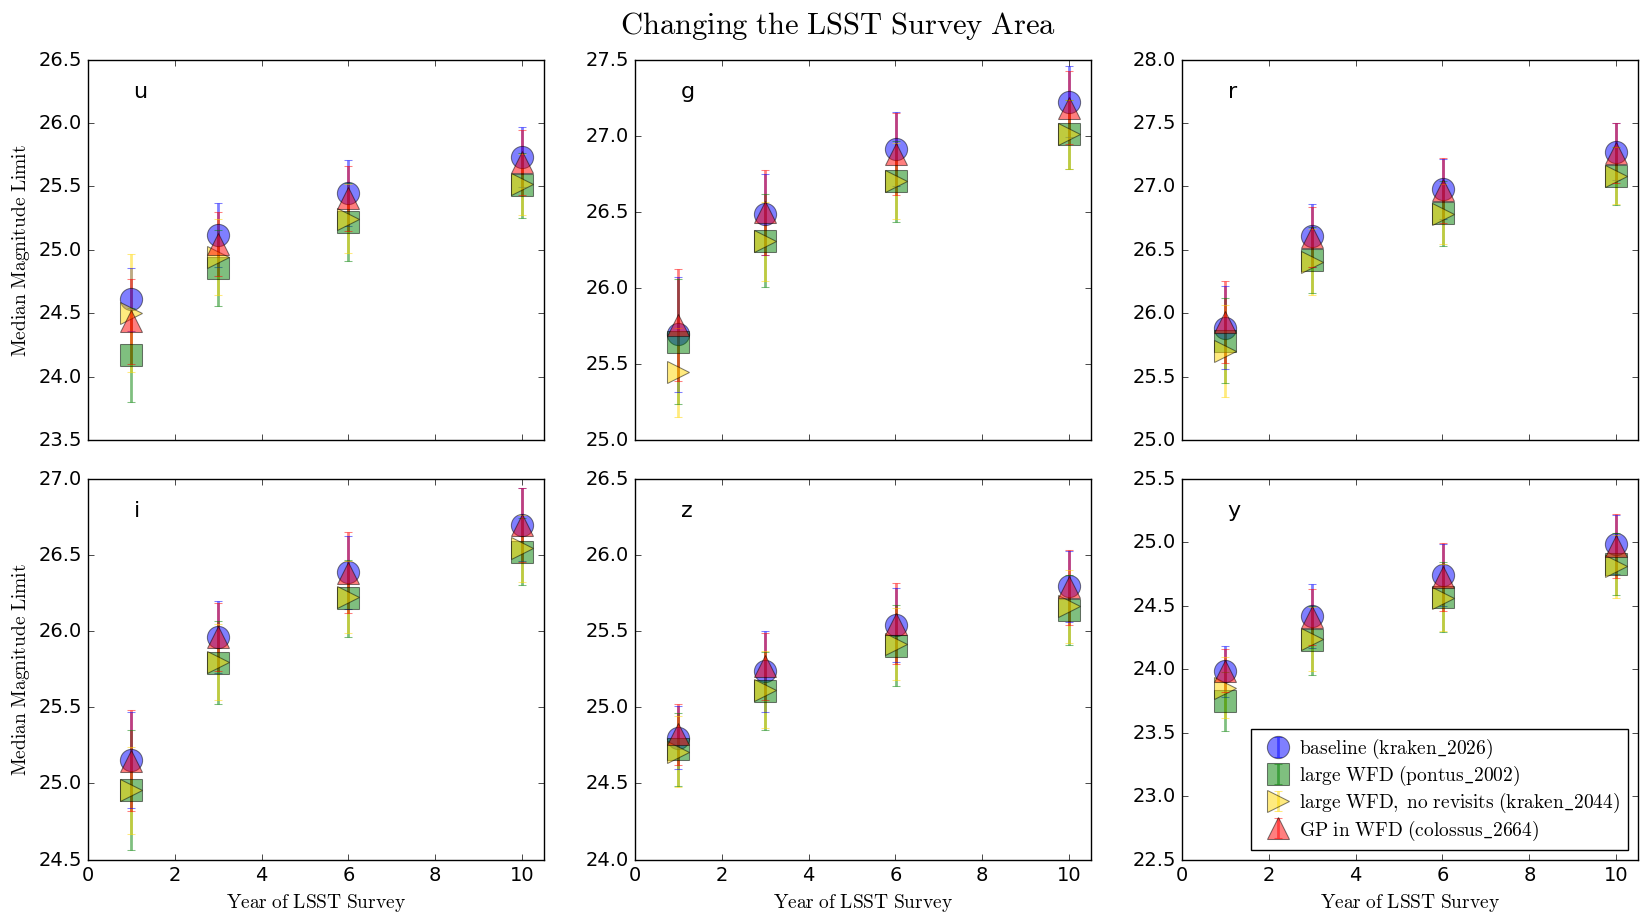
\includegraphics[width=15cm,trim={0cm 0cm 0cm 0cm}, clip]{figures/maglims_area.png}
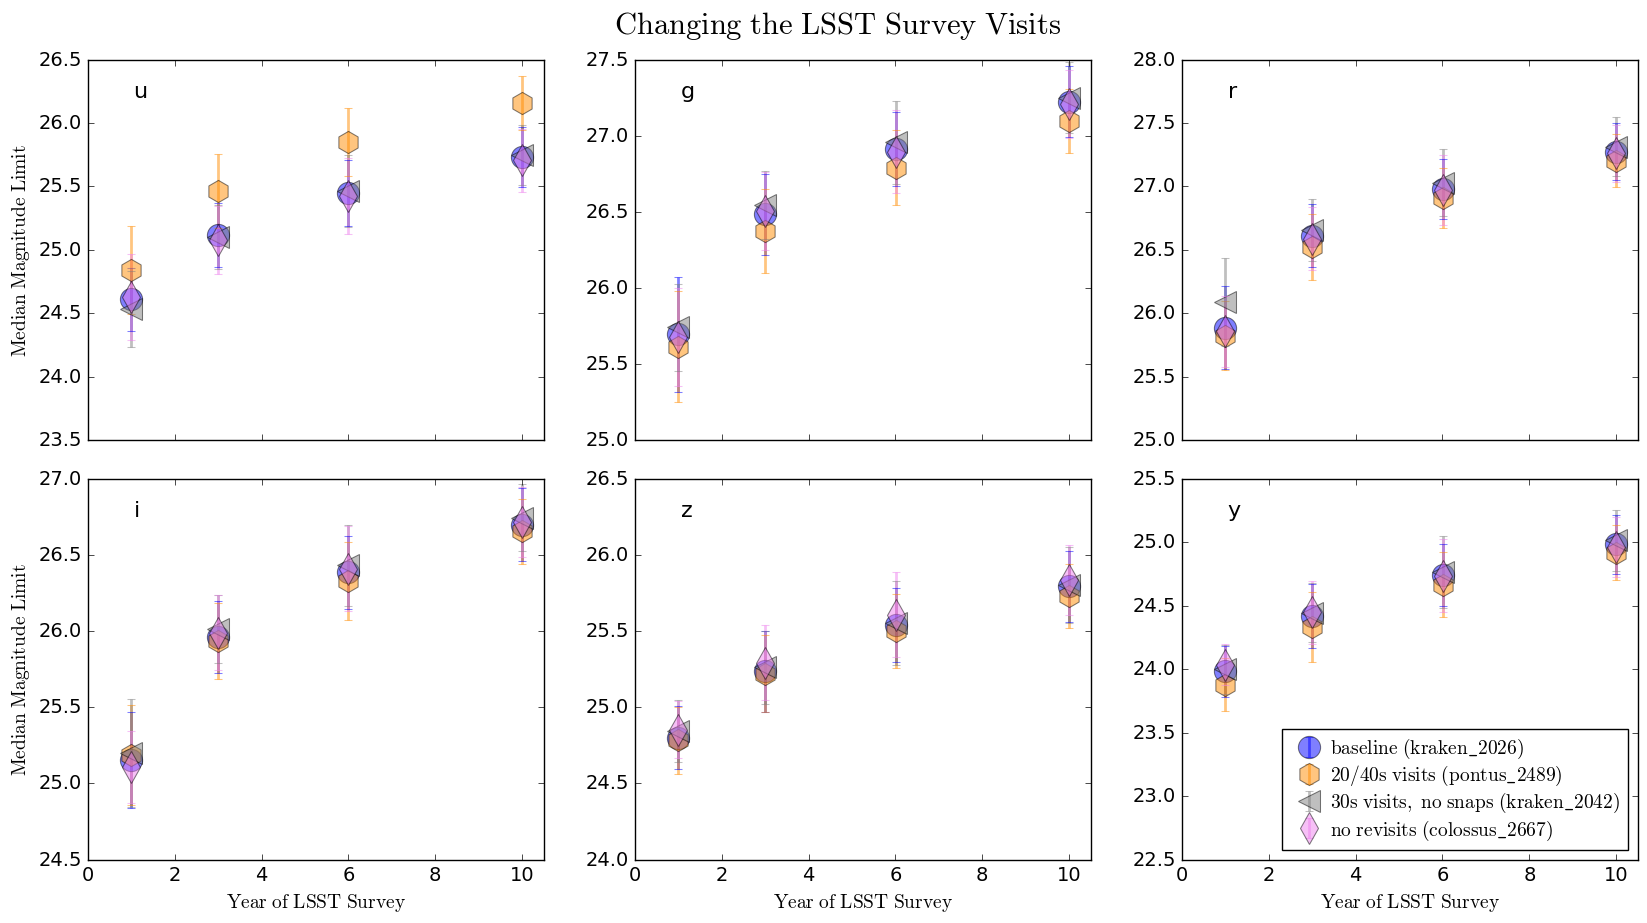
\includegraphics[width=15cm,trim={0cm 0cm 0cm 0cm}, clip]{figures/maglims_visits.png}
\caption{The median 5$\sigma$ magnitude limit for all fields with at least one visit in three filters, as a function of survey year, for LSST filters $ugrizy$ (top left to bottom right panel in each 3x2 panel set). The baseline survey, {\tt kraken\_2026}, is shown with blue circles in each set. The magnitude limit evolution over the 10 year survey is demonstrated for OpSim runs that change the survey area (top) or change the visit strategy (bottom). Results for rolling cadences are shown in Figure \ref{fig:maglims_2}. This plot demonstrates that the overall evolution in photometric quality is similar to the baseline for the majority of the OpSim runs. The two runs that differ the most from the baseline are {\tt pontus\_2002}, in which the WFD survey area is extended at the expense of depth per field (green squares, top), and {\tt pontus\_2489}, in which the $u$-band filter is done with $40$-second exposures and all other filters with $20$-second exposures (orange hexagons, bottom). \label{fig:maglims}}
\end{center}
\end{figure*}

\begin{figure*}
\begin{center}
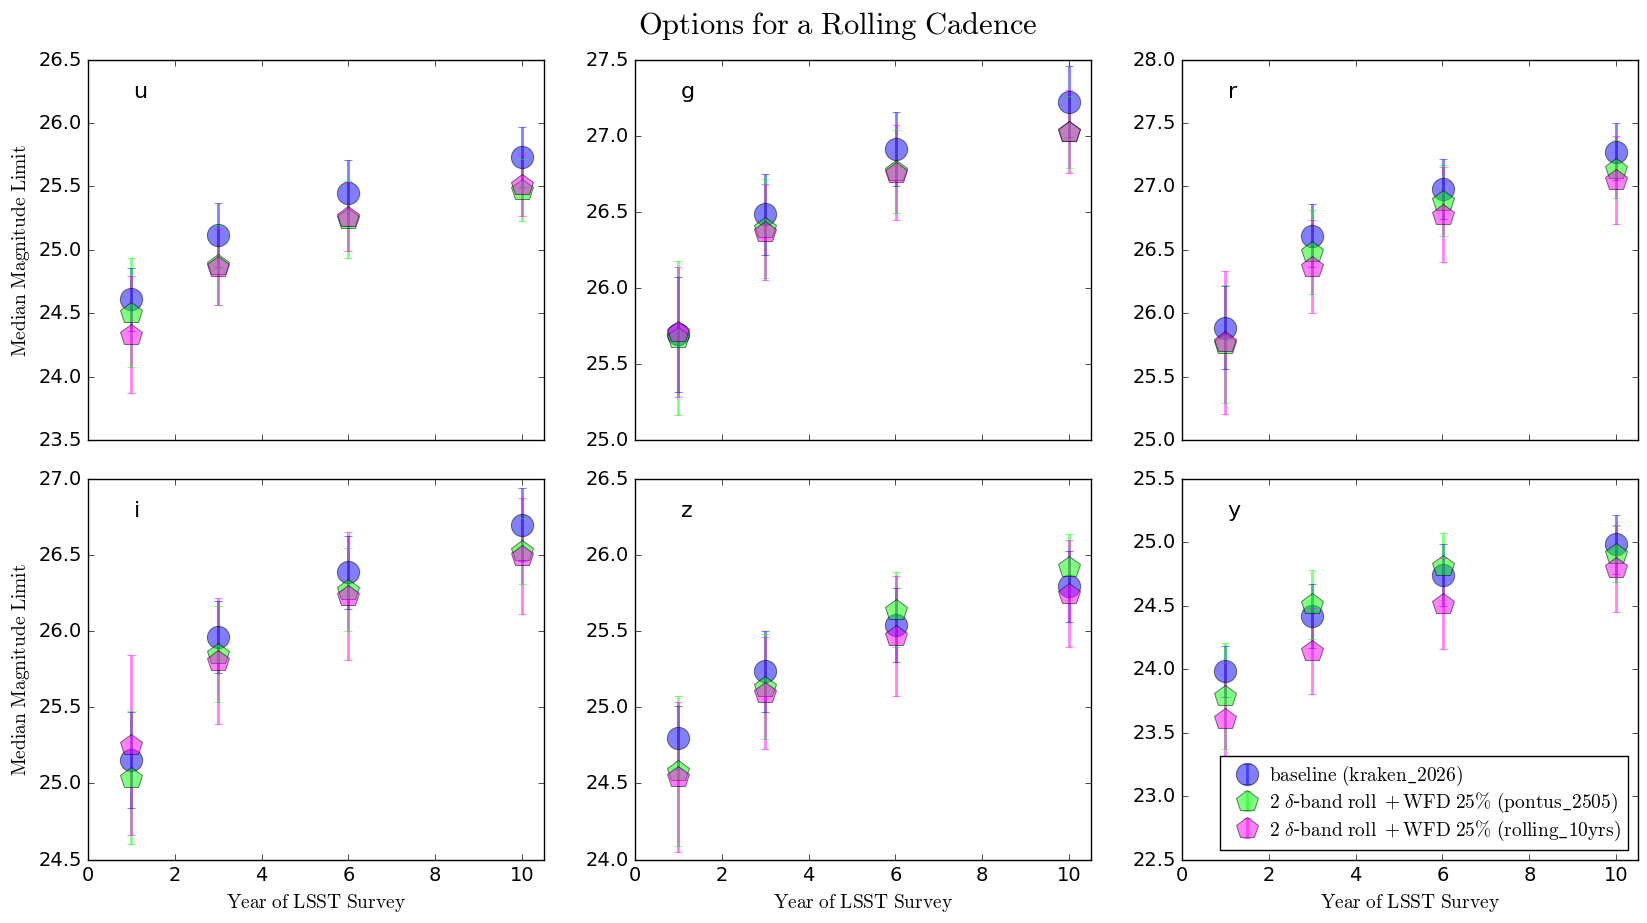
\includegraphics[width=15cm,trim={0cm 0cm 0cm 0cm}, clip]{figures/maglims_roll_3.png}
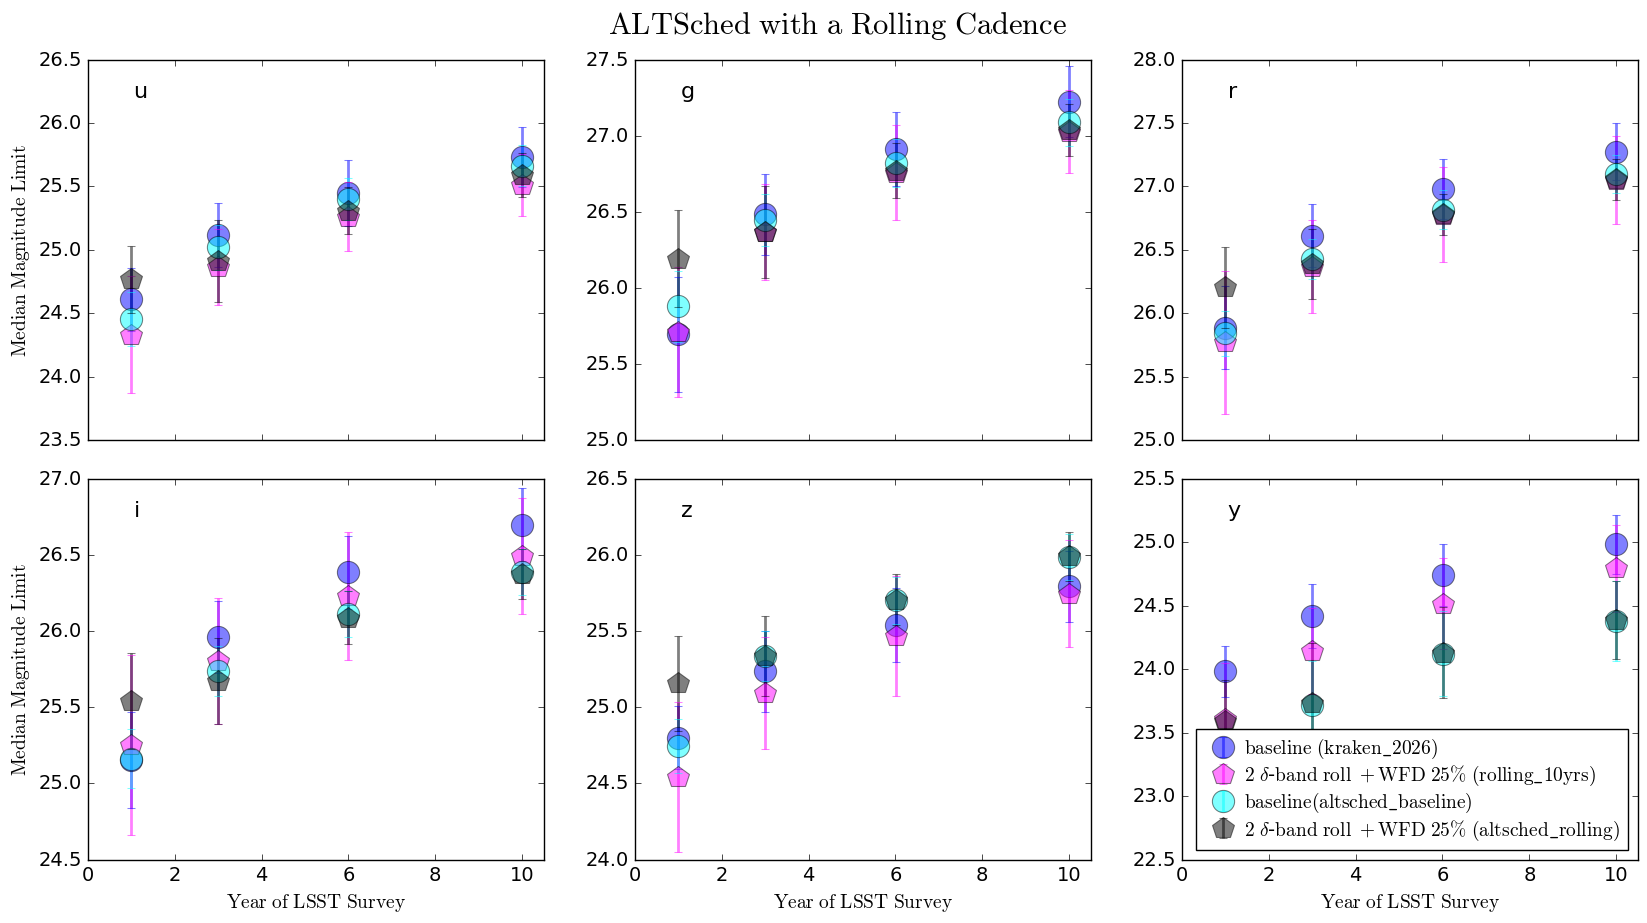
\includegraphics[width=15cm,trim={0cm 0cm 0cm 0cm}, clip]{figures/maglims_roll_4.png}
\caption{Similar to Figure \ref{fig:maglims}, but for a strategy that adopts a rolling cadence over the baseline WFD area of $18,000$ square degrees: two bands of declination, each prioritized in alternating years, while the deprioritized band gets 25\% of the baseline number of visits. Recall that {\tt pontus\_2502} has a bug that limited the number of visits and is shown only for reference in the top plot (lime green pentagons); {\tt rolling\_10yrs} is the OpSim database used to represent a rolling cadence option in this analysis (magenta pentagons). In the bottom plot, we compare to the results of the {\tt ALTSched}, without and with a rolling cadence (cyan circles and black pentagons, respectively). These two plots demonstrate that the overall evolution in photometric quality for rolling cadence options is not equivalent to the baseline's uniform progression cadence (blue circles). Also keep in mind that the median magnitudes for a rolling cadence with two declination bands only applies to half of the sky area compared to the baseline, which is a drawback of this kind of rolling cadence that is not expressed by this plot. \label{fig:maglims_2}}
\end{center}
\end{figure*}

{\bf Summary --} As demonstrated above, it turns out that many of the {\tt OpSim} runs result in a similar evolution for the median limiting magnitude for each filter as a function of survey year, and thus would not produce different photo-$z$ results, except for these three: {\tt pontus\_2002}, which has a larger WFD survey area of $24700$ square degrees ($-78 < \delta < +18$); {\tt pontus\_2489}, which does $20$-second visits in $grizy$ filters and $40$-second visits in $u$-band, increasing the $u$-band depth and leading to a larger total number of visits in the others filters; and {\tt rolling\_10yrs}, a rolling cadence that alternates between two bands of declination. We will only simulate photo-$z$ results for those three {\tt OpSim} runs, plus the {\tt OpSim} baseline, and the {\tt ALTSched} baseline and rolling cadence.


% % % % % % % % % % % % % % % % % % % % % % % % % % % % %
\subsection{The CMNN Photo-$z$ Estimator}\label{ssec:pz_exp_cmnn}

For this work we have used the color-matched nearest-neighbors (CMNN) photometric redshift estimator from \cite[][herafter G18]{2018AJ....155....1G}. The CMNN should not be taken as representing the ``best" photo-$z$ estimator or the ``official" LSST algorithm -- it is neither of these things. It is a simple algorithm that produces photo-$z$ results of a statistical quality that directly correlates with the photometric quality of the input, and thus is very useful for evaluating the impact on photo-$z$ of any changes to the LSST photometric quality -- such as the {\tt OpSim} runs that we consider in this work.

As described in G18, this estimator uses a training set of galaxies with known redshifts and a test set for which photo-$z$ are to be estimated. For each galaxy in the test set, the estimator first identifies a color-matched subset of training galaxies by calculating the Mahalanobis distance in color-space between the test galaxy and all training-set galaxies. The Mahalanobis distance in this case is the difference between the test- and training-set galaxy color, divided by the photometric error of the test-set galaxy color, summed over all available colors (Equation 1 in G18). Then, a threshold value is applied that defines a ``good" color match. This threshold is set by the percent point function (PPF): for example, for $N_{\rm dof}=5$, PPF$=95$ per cent of all training galaxies consistent with the test galaxy will have $D_M < 11.07$ (where $N_{\rm dof}$, the number of degrees of freedom, is the number of colors). The estimator then chooses one of the color-matched training-set galaxies (e.g. the nearest-neighbor or a random selection), and uses that galaxy's known redshift as the test-set galaxy's photo-$z$ (a "redshift donor"). The uncertainty in the photo-$z$ estimate is taken to be the standard deviation of the true redshifts of training-set galaxies in the color-matched subset. 

Compared to G18, there are some minor differences in how this photo-$z$ estimator was applied in this work. Here, we require that a test-set galaxy be detected in the LSST filters $griz$ and thus have colors $g-r$, $r-i$, and $i-z$ or else a photo-$z$ estimate is not attempted, and we've used a threshold of PPF=$0.68$ to define the color-matched subset of training galaxies. Unlike G18, we choose randomly from the color-matched subset of training galaxies instead of choosing the nearest neighbor. This difference leads to less accurate and less precise photometric redshifts, but by using a random selection in the photo-$z$ estimator, the {\tt OpSims} runs that degrade/enhance the LSST photometry end up having a larger relative impact on the resulting photometric redshifts. This helps with the experiment at hand, which is to assess the relative impacts of different {\tt OpSim} runs, and {\em not} to generate the best possible photo-$z$ results for each {\tt OpSim} run.

As a final note, to accelerate processing time, we have applied both the color and magnitude pre-cuts to the training set, as described in G18. The color cut is fairly benign, but the magnitude pre-cut effectively works as a ``pseudo-prior" by cutting down the training set to the 10\% of training galaxies with an $i$-band magnitude nearest to the test galaxy's $i$-band magnitude. The ``pseudo-prior" may improve accuracy of the photo-$z$ estimate for some, but can also introduce a bias in the results. Since all of the experiments in this work will be looking at {\it relative} changes to the photo-$z$ quality as various inputs are changed, this kind of degradation to the {\it absolute} photo-$z$ quality is acceptable in this case.


% % % % % % % % % % % % % % % % % % % % % % % % % % % % %
\subsection{Simulating LSST Photometry for the Training and Test Catalogs} \label{ssec:pz_exp_cats}

For this work we use the same simulated mock galaxy catalog as used in G18. This catalog contains the ``true" redshift and the ``true" apparent magnitudes in $ugrizy$ for all galaxies. The training and test set galaxies are drawn randomly from this catalog. We use $1\times10^6$ galaxies for the training set, and $5\times10^4$ galaxies for the test set. Justification for the sizes of the test and training sets is provided in G18, but here we note that the size of the test set is adequate to achieve statistical measures in the high-$z$ bins.

For the training set, we simulate observed apparent magnitudes for all galaxies assuming that the $5{\sigma}$ photometric depths in each filter are equivalent to the LSST baseline 10-year survey: $u=26.09,g=27.38,r=27.53,i=26.83,z=26.06,y=24.86$. This is the same as what was used in G18. For the test set, we also simulate observed apparent magnitudes for all galaxies using the $5{\sigma}$ photometric depths in each filter, but these depths change for the different LSST observing strategies that we consider in this work. We randomly assign each test galaxy to one of the simulated ``fields" from our MAF, as described above in Section \ref{ssec:pz_opsim_phot}. For all training- and test-set galaxies, once we know the $5{\sigma}$ photometric depth to apply, we derive the expected photometric error based on each galaxy's ``true" catalog magnitude (using Equation 5 from \citealt{2008arXiv0805.2366I}), and then add a random scatter proportional to this uncertainty to simulate observational uncertainties. This method is described in more depth, with plots of error {\it vs.} apparent magnitude, in G18.

In all of our experiments, both the test and training sets are limiting to $i<25$ mag, so that we are simulating photo-$z$ for samples of ``good" galaxies. Furthermore, in our implementation of the CMNN algorithm, galaxies are required to have at least 3 colors or else a photo-$z$ estimate is not attempted. Thus, our results represent the photo-$z$ quality of a ``gold'' sample of galaxies for cosmological analyses, and do not reflect any impact on the survey area or number of galaxies available for a cosmological analyses -- only the photo-$z$ quality of the ``best'' observed galaxies.


% % % % % % % % % % % % % % % % % % % % % % % % % % % % %
\subsection{Analysis Methodology}\label{ssec:pz_exp_meth}

We take these blurbs from G18 to describe our statistical measures of photo-$z$ quality and the common plot styles that we will use to represent our results. For this analysis we will use only the point estimates of photo-$z$ for each of our test galaxies, although CMNN is capable of returning a full posterior (e.g., Schmidt et al. 2018, in prep.). Although we have included simulated galaxies with $z<0.3$ and $z>3$ in both the test and training sets, our analysis focuses on a cosmological set of galaxies with $0.3 \leq z_{\rm phot} \leq 3$.

{\bf Statistical Measures --} Where $z_{\rm true}$ is the ``true" catalog redshift and $z_{\rm phot}$ is the photo-$z$, the error is $\Delta z_{(1+z)} = (z_{\rm true} - z_{\rm phot})/(1+z_{\rm phot})$. Including a factor of $(1+z)$ in the denominator acts to compensate for larger uncertainties at high-$z$. For all of our results we calculate the robust standard deviation in $\Delta z_{(1+z)}$ as the FWHM of the interquartile range (IQR) divided by $1.349$ ($\sigma_{\rm IQR}$) and the robust bias as the mean value of $\Delta z_{(1+z)}$ in the IQR ($\overline{\Delta z_{\rm(1+z), IQR}}$). We reject catastrophic outliers ($|z_{\rm spec}-z_{\rm phot}| > 1.5$) from the IQR before calculating the standard deviation and bias, {\em which is different from our analyses in past work} such as \cite{2018AJ....155....1G}. We bootstrap our uncertainties on these statistical measures by randomly drawing a subsets and recalculating the statistics 1000 times. Outlier galaxies are identified as those with $\Delta z_{(1+z)} > 3\sigma_{\rm IQR}$ or $\Delta z_{(1+z)} > 0.06$, whichever is {\it larger}, where $\sigma_{\rm IQR}$ is calculated from all galaxies in $0.3 \leq z_{\rm phot} \leq 3.0$ (i.e., outliers are defined globally). The fraction of outlier galaxies that we calculate {\it includes} catastrophic outliers (as defined above).

{\bf Plot Styles --} To visualize our photo-$z$ results we create plots that compare the true $vs.$ photometric redshifts, in which outlier galaxies are typically colored red and a solid line of $z_{\rm true} = z_{\rm phot}$ is drawn to guide the eye. These plots are useful to obtain a global sense of the photo-$z$ quality and the structure in the outliers positions, especially the features that are perpendicular to the $z_{\rm true} = z_{\rm phot}$, which represent photo-$z$ degeneracies caused by the Balmer break passing between filters. We also plot the robust standard deviation, robust bias, and fraction of outliers as a function of $z_{\rm phot}$, typically as a way to directly compare the bulk photo-$z$ results of experiments in which the simulated galaxy photometry has been altered in some way. 


% % % % % % % % % % % % % % % % % % % % % % % % % % % % %
\subsection{Results}\label{ssec:pz_results}

As discussed in Section \ref{ssec:pz_opsim_phot}, only three of the {\tt OpSim} runs result in a significantly different evolution in the median photometric depth of WFD fields compared to the baseline, and so we only simulate photo-$z$ results for the following: 

\begin{itemize}
\item {\tt OpSim} {\tt kraken\_2026}, the baseline run
\item {\tt OpSim} {\tt pontus\_2002}, a larger WFD survey area of $24700$ square degrees ($-78 < \delta < +18$)
\item {\tt OpSim} {\tt pontus\_2489}, $20$-second visits in $grizy$ filters and $40$-second visits in $u$-band, increasing the $u$-band depth and leading to a larger total number of visits in the others filters
\item {\tt OpSim} {\tt rolling_10yrs}, a rolling cadence that alternates between two bands of declination
\item {\tt ALTSched} {\tt altched\_baseline}, the baseline run
\item {\tt ALTSched} {\tt altsched\_rolling}, a rolling cadence that alternates between two bands of declination
\end{itemize}

In Figure \ref{fig:tzpz} we plot the true {\it vs.} the photometric redshifts at years $1$, $3$, and $10$ of the LSST survey, for each of the four {\tt OpSim} runs considered in this work. While the improvement over the years of the survey is easily noticed in these plots (compare columns), very little distinction is visible in the photo-$z$ results for the different {\tt OpSim} runs (compare rows). For this reason, we do not include the {\tt ALTSched} results in this format. The following plots of statistical measures are more useful in this regard.

In Figure \ref{fig:stats_opsim} we compare the statistical measures of robust standard deviation and bias from the IQR (after the rejection of catastrophic outliers), and the fraction of outliers (including catastrophic) as a function of photo-$z$ bin for each of the four considered {\tt OpSim} runs, at $1$ and $10$ years of the LSST survey. We draw the following conclusions from Figure \ref{fig:stats_opsim}. 
\begin{itemize}
\item Extending the survey area to $-78 < \delta < +18$ for a large WFD area of $24,700$ square degrees (green line; {\tt pontus\_2002}) results in degraded photo-$z$ quality compared to the baseline (blue line; {\tt kraken\_2026}). This degradation is most clearly seen in redshift bins $1.5 \lesssim z_{\rm phot} \lesssim 2.2$ at 1 year.
\item The 20/40s "many visits" option that lengthens the $u$-band exposure time to $40$ seconds and shortens it to $20$ seconds in $grizy$ (orange line; {\tt pontus\_2489}) performs similarly to the baseline, but with a small but significant improvement in the standard deviation and fraction of outliers at $z_{\rm phot} \gtrsim 1.5$.
\item The rolling cadence that alternates between two declination bands ({\tt rolling\_10yrs}; magenta line) produces degraded results that are similar to those from extending the total WFD area (green line).
\end{itemize}

In Figure \ref{fig:stats_altsched} we compare the statistical measures of robust standard deviation and bias from the IQR (after the rejection of catastrophic outliers), and the fraction of outliers (including catastrophic) as a function of photo-$z$ bin for the {\tt OpSim} baseline and rolling cadence to the {\tt ALTSched} baseline and rolling cadence. We draw the following conclusions from Figure \ref{fig:stats_altsched}. 
\begin{itemize}
\item The {\tt OpSim} and {\tt ALTSched} baselines deliver equivalent results in terms of photo-$z$ quality.
\item The {\tt ALTSched} rolling cadence delivers the better photo-$z$ at year 1 across all redshift bins than the {\tt OpSim} rolling cadence, or either simulator's baseline. We attribute this to the fact that {\tt ALTSched}'s rolling cadence does not spend any time observing the deprioritized declination band, whereas {\tt OpSim}'s {\tt rolling\_10yrs} allows it $25\%$ of the baseline number of visits.
\item Of these four simulations, the {\tt OpSim} baseline cadence delivers the best photo-$z$ at year 10.
\end{itemize}

In Figure \ref{fig:evol} we chart the evolution in the statistical measures over year of the survey in redshift bins of $0.8 \leq z_{\rm phot} \leq 1.2$  and $1.8 \leq z_{\rm phot} \leq 2.2$. We can see that all four {\tt OpSim} runs progress in a similar fashion {\it except} for the rolling cadence with two declination bands done in alternating years (magenta line; {\tt rolling\_10yrs}), which shows a mild improvement at year 1 (but recall the improved statisics would only apply to half of the sky area). The {\tt ALTSched} rolling cadence shows an even more pronounced improvement at year 1, but by year 10 is consistent with the baseline cadence.

In Table \ref{tab:zbins} we provide the relative robust standard deviation results in two redshift bins, $0.3<z_{\rm phot}<1.5$ and $1.5<z_{\rm phot}<3.0$, for years 1, 3, 6, and 10, for each of the considered {\tt OpSim} and {\tt ALTSched} runs. Note that these redshift bins are not the same as those used for Figure \ref{fig:evol}. These results are reported as {\it relative to} the baseline robust standard deviation for the low-$z_{\rm phot}$ bin at LSST year 10 (i.e., all values of the robust standard deviation are divided by this value). Note that the ``many visits" survey ({\tt pontus\_2489}) {\it performs better than the {\tt OpSim} baseline in the high-$z$ bin for all years}, and has an equivalent performance to the baseline in the low-$z$ bin.

\begin{figure}
\begin{center}
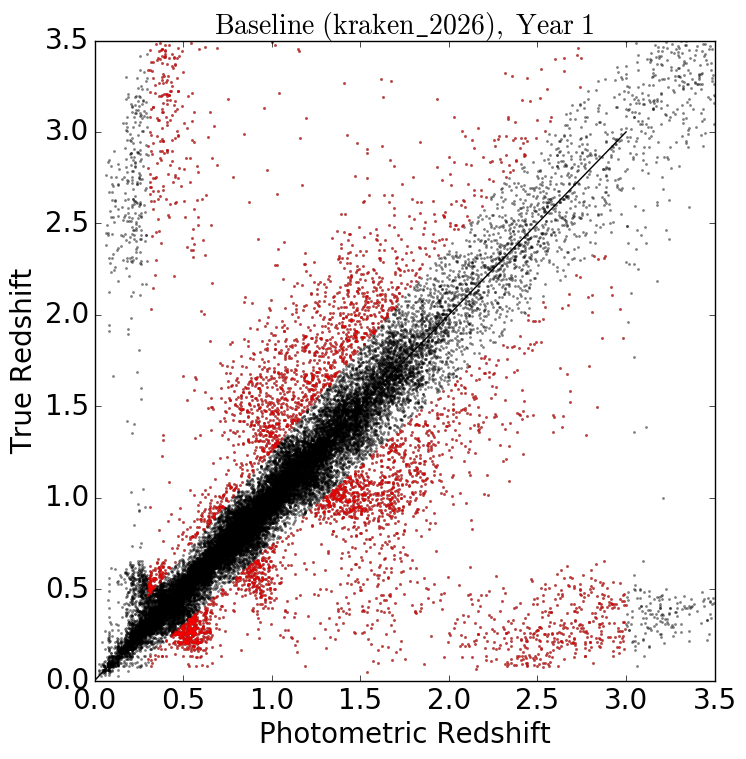
\includegraphics[width=4.5cm,trim={0cm 0cm 0cm 0cm},clip]{figures/tzpz_kraken2026_1.png}
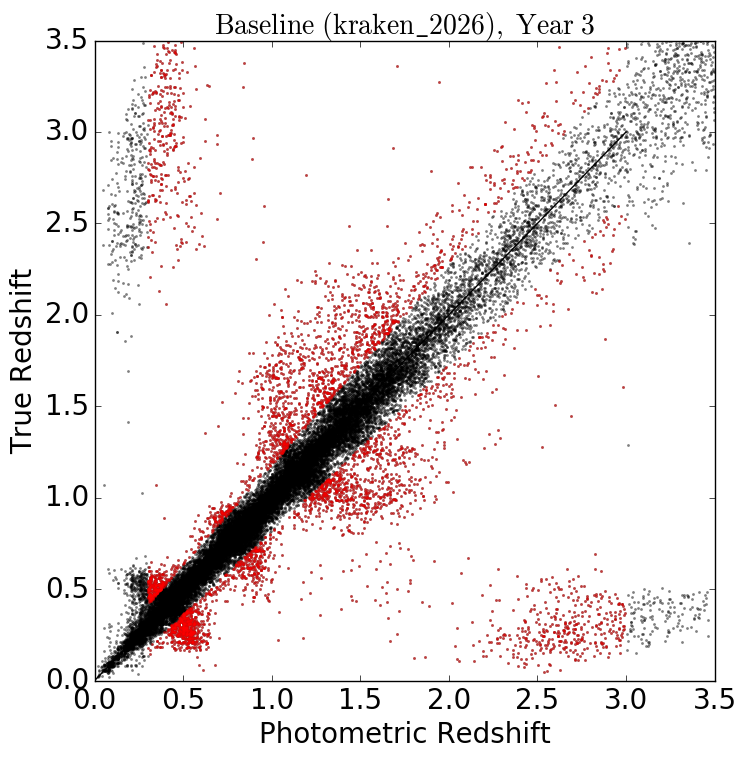
\includegraphics[width=4.5cm,trim={0cm 0cm 0cm 0cm},clip]{figures/tzpz_kraken2026_3.png}
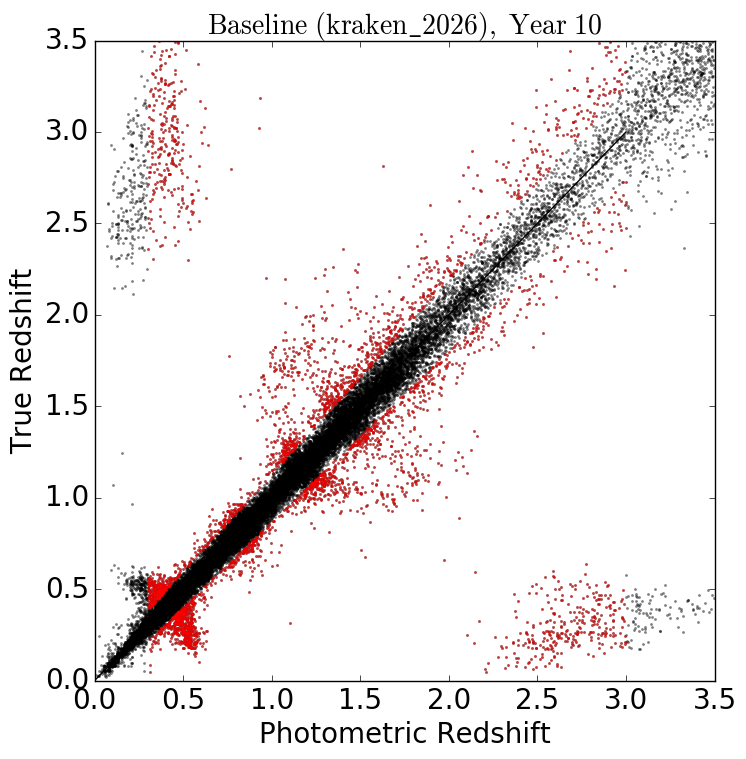
\includegraphics[width=4.5cm,trim={0cm 0cm 0cm 0cm},clip]{figures/tzpz_kraken2026_10.png}
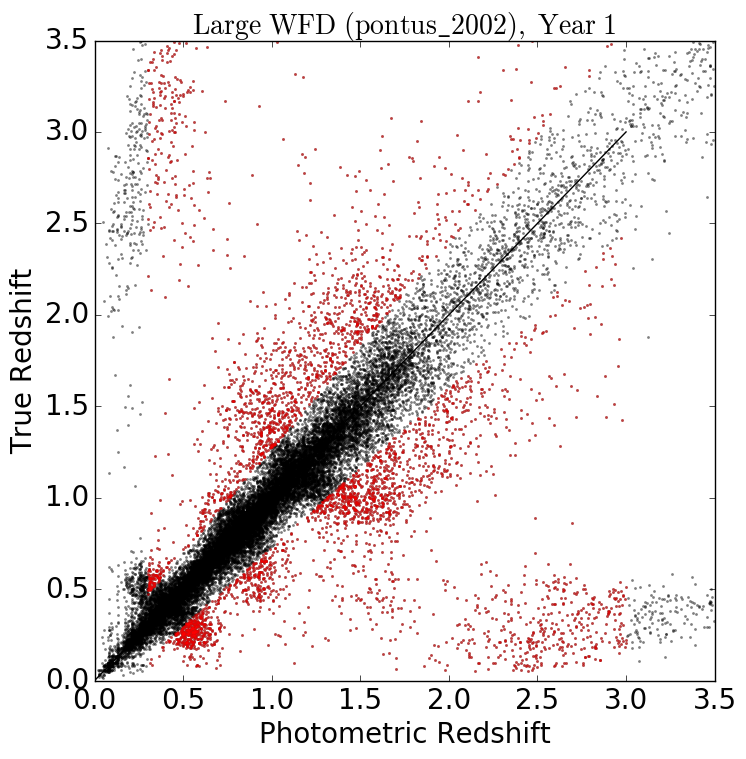
\includegraphics[width=4.5cm,trim={0cm 0cm 0cm 0cm},clip]{figures/tzpz_pontus2002_1.png}
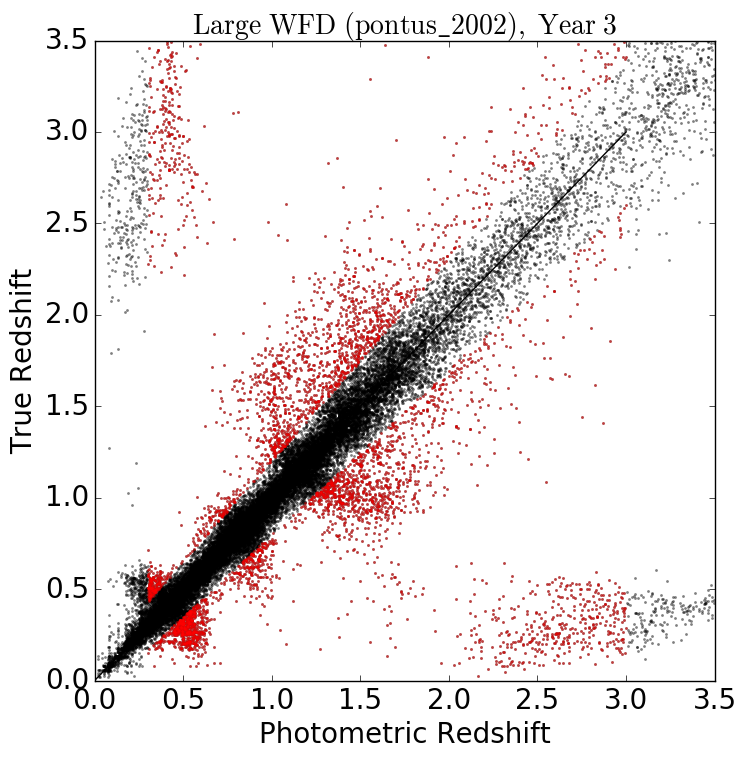
\includegraphics[width=4.5cm,trim={0cm 0cm 0cm 0cm},clip]{figures/tzpz_pontus2002_3.png}
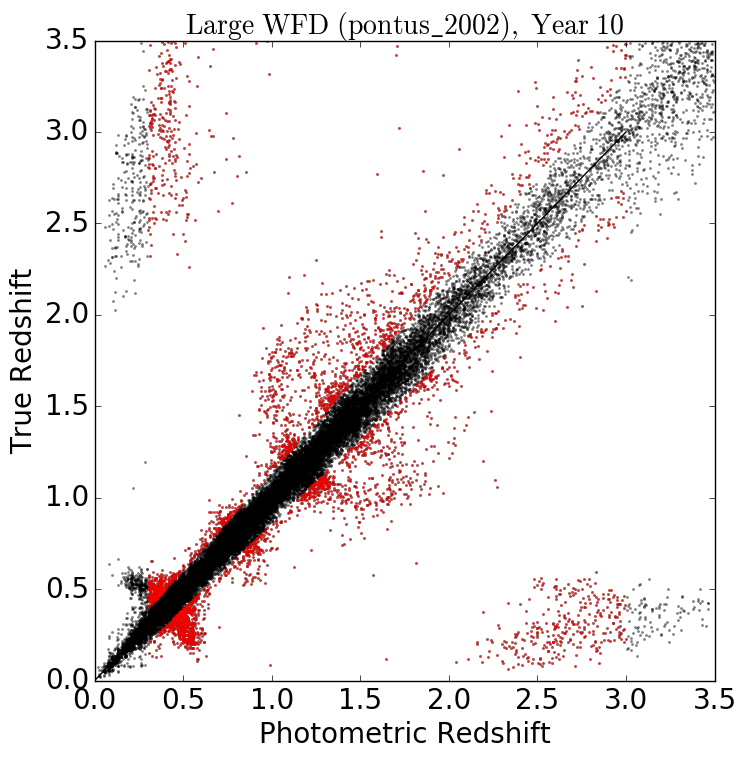
\includegraphics[width=4.5cm,trim={0cm 0cm 0cm 0cm},clip]{figures/tzpz_pontus2002_10.png}
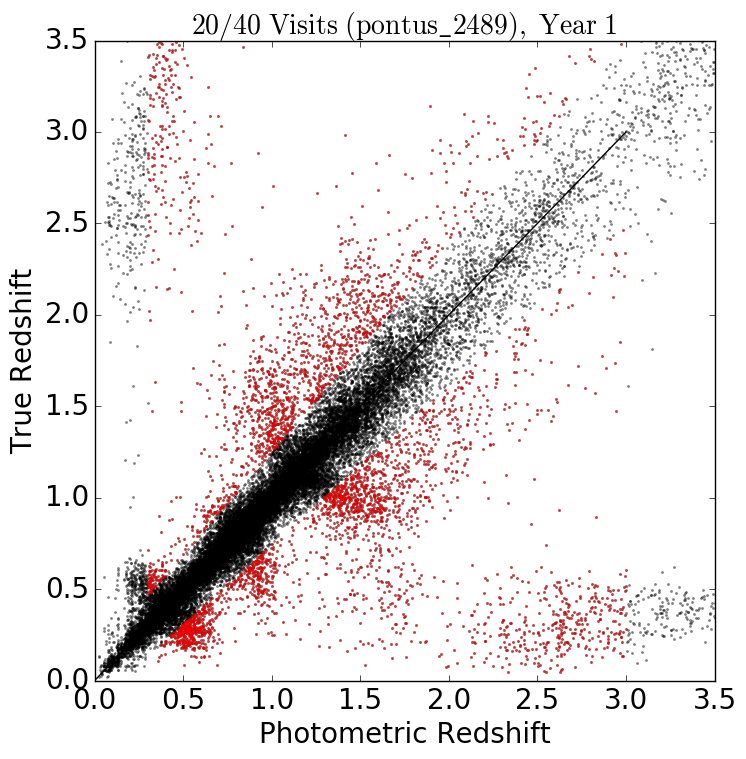
\includegraphics[width=4.5cm,trim={0cm 0cm 0cm 0cm},clip]{figures/tzpz_pontus2489_1.png}
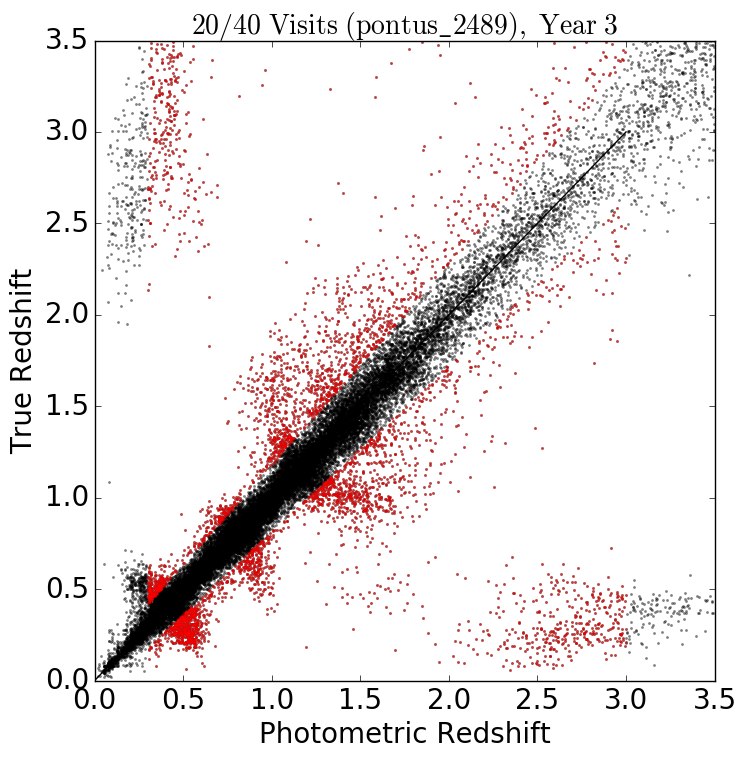
\includegraphics[width=4.5cm,trim={0cm 0cm 0cm 0cm},clip]{figures/tzpz_pontus2489_3.png}
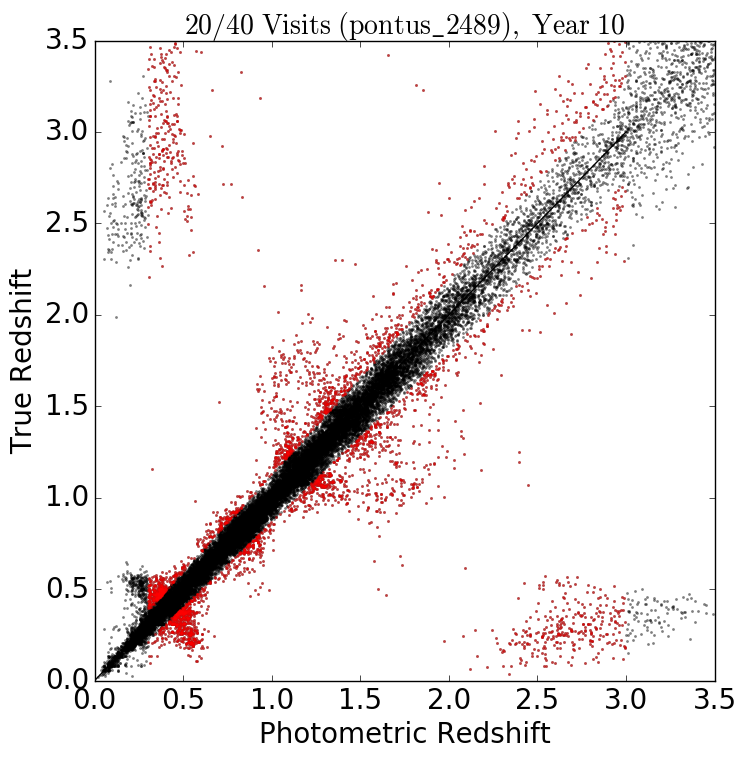
\includegraphics[width=4.5cm,trim={0cm 0cm 0cm 0cm},clip]{figures/tzpz_pontus2489_10.png}
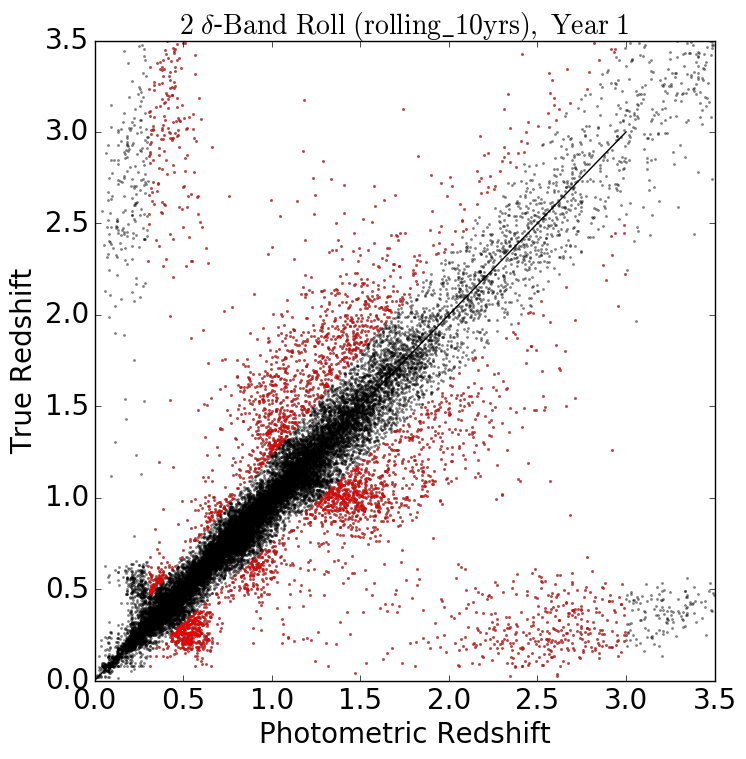
\includegraphics[width=4.5cm,trim={0cm 0cm 0cm 0cm},clip]{figures/tzpz_rolling10yrs_1.png}
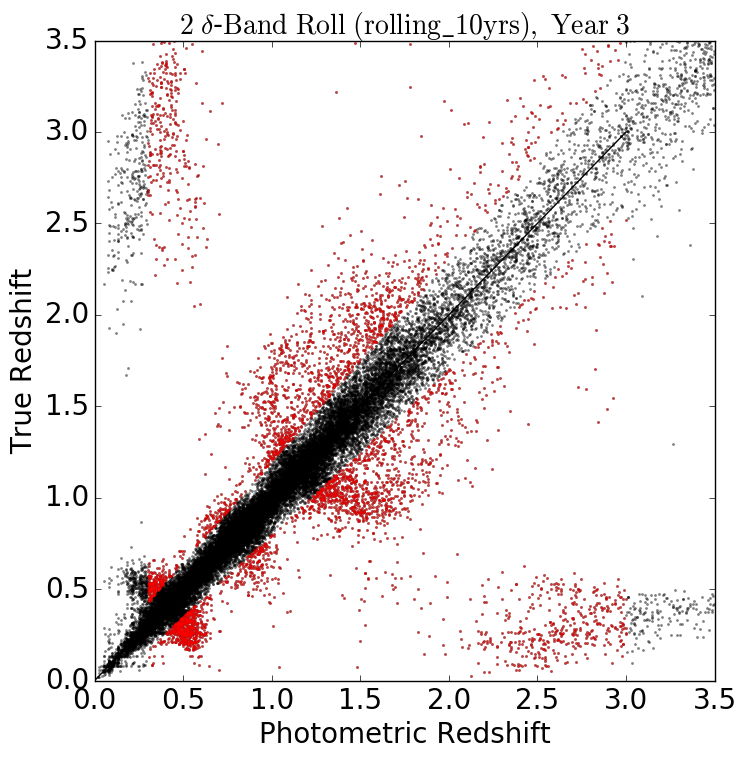
\includegraphics[width=4.5cm,trim={0cm 0cm 0cm 0cm},clip]{figures/tzpz_rolling10yrs_3.png}
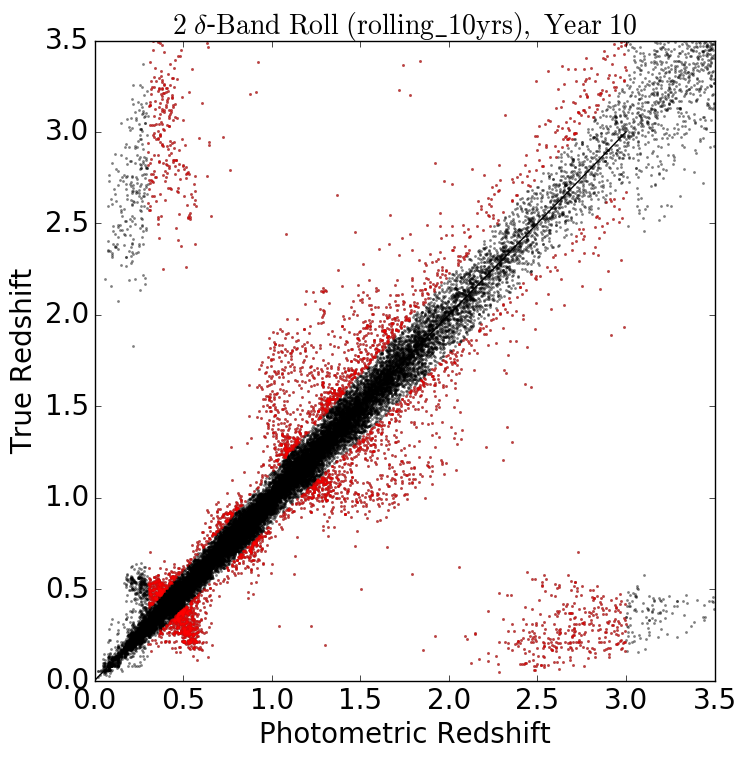
\includegraphics[width=4.5cm,trim={0cm 0cm 0cm 0cm},clip]{figures/tzpz_rolling10yrs_10.png}
\caption{True {\it vs.} photometric redshifts for all test galaxies, with statistical outliers plotted as red points. Columns from left to right represent results at years 1, 3, and 10. Rows from top to bottom represent results from the {\tt OpSim} baseline ({\tt kraken\_2026}), large WFD area with declinations including  $-78<\delta<+18$ degrees ({\tt pontus\_2002}), the ``many visits" strategy with 40/20 second exposures in $u$/$grizy$ filters ({\tt pontus\_2489}), and a rolling cadence with two declination bands ({\tt rolling\_10yrs}). Results from {\tt ALTSched} are not plotted in this way. \label{fig:tzpz}}
\end{center}
\end{figure}

\begin{figure}
\begin{center}
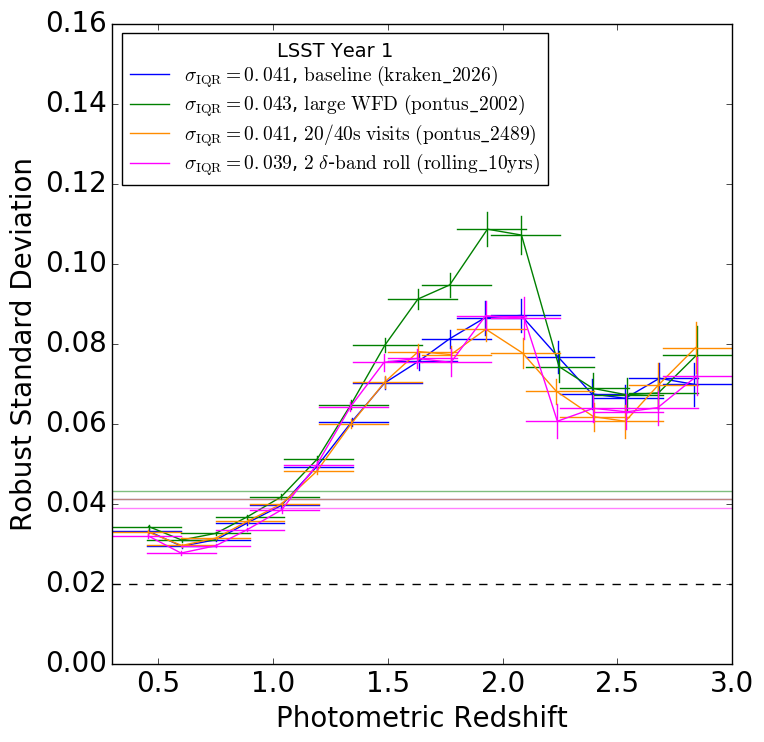
\includegraphics[width=6cm,trim={0cm 0cm 0cm 0cm},clip]{figures/year1_IQRs.png}
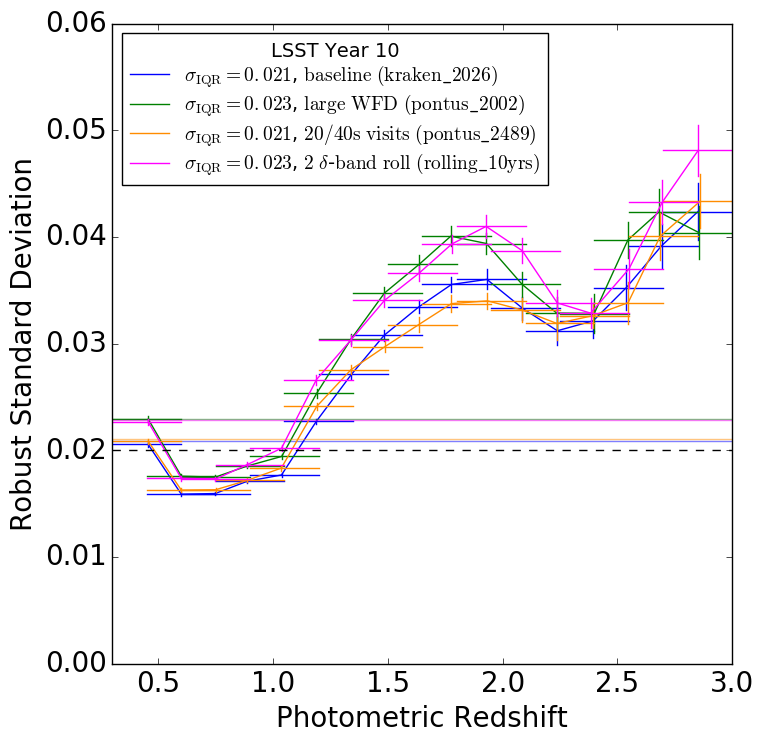
\includegraphics[width=6cm,trim={0cm 0cm 0cm 0cm},clip]{figures/year10_IQRs.png}
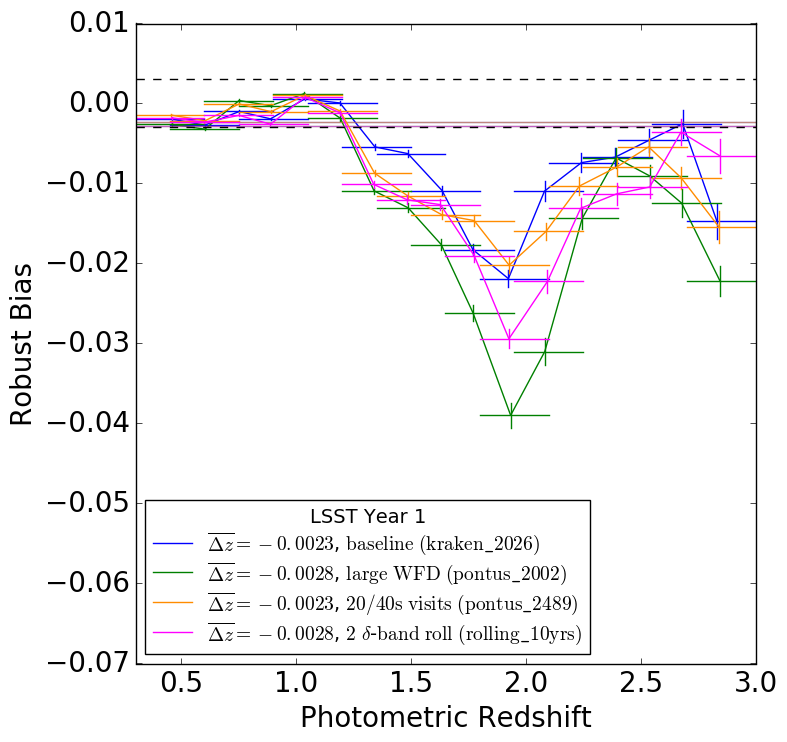
\includegraphics[width=6cm,trim={0cm 0cm 0cm 0cm},clip]{figures/year1_bias.png}
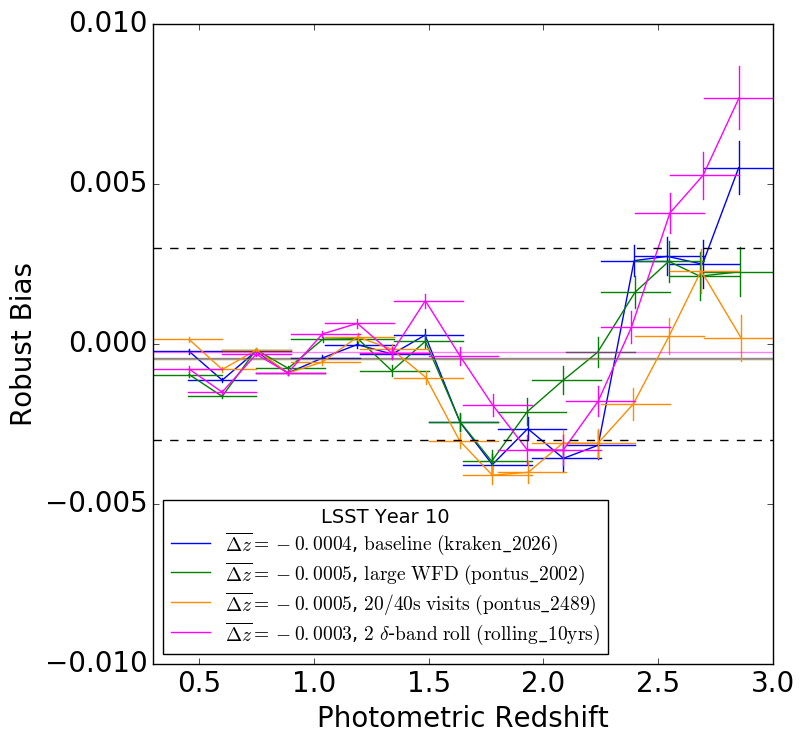
\includegraphics[width=6cm,trim={0cm 0cm 0cm 0cm},clip]{figures/year10_bias.png}
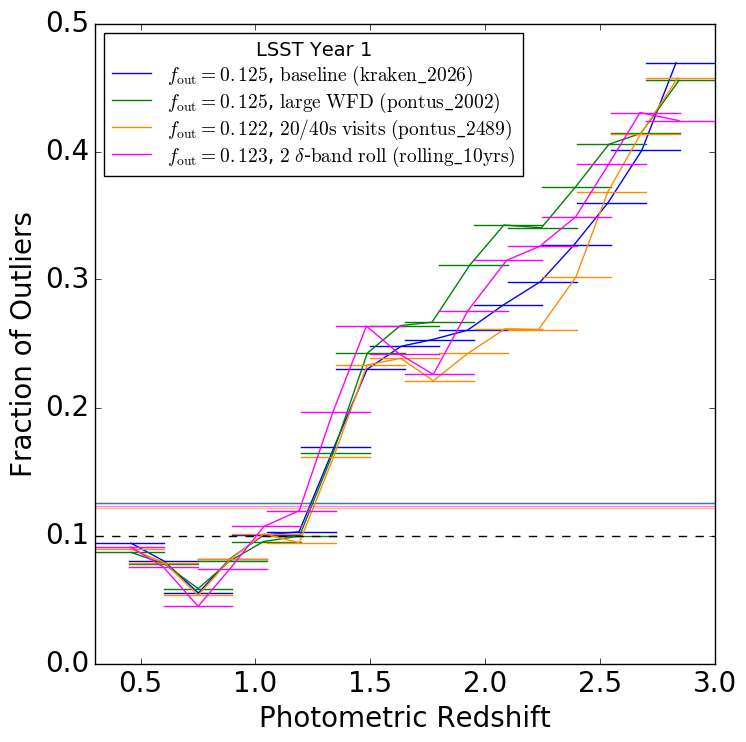
\includegraphics[width=6cm,trim={0cm 0cm 0cm 0cm},clip]{figures/year1_fout.png}
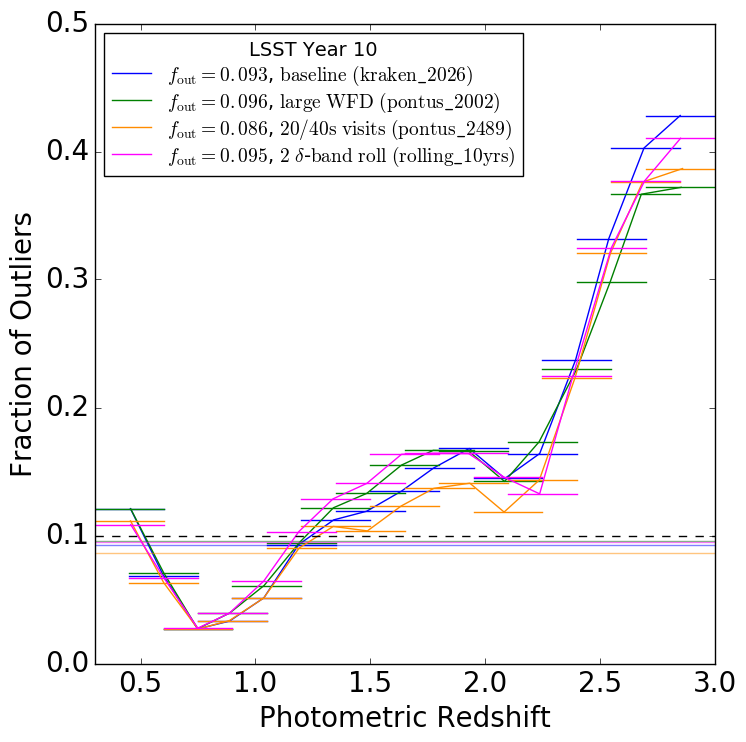
\includegraphics[width=6cm,trim={0cm 0cm 0cm 0cm},clip]{figures/year10_fout.png}
\caption{Statistical measures of robust standard deviation (from the IQR; top), robust bias (middle), and fraction of outliers (bottom) as a function of photo-$z$, at years $1$ (left column) and $10$ (right column). Note that the $y$-axes are not matched between columns. Results are presented for the baseline ({\tt kraken\_2026}; blue), large WFD area with declinations including  $-78<\delta<+18$ degrees ({\tt pontus\_2002}; green), the ``many visits" strategy with 40/20 second exposures in $u$/$grizy$ filters ({\tt pontus\_2489}; orange), and a rolling cadence with two declination bands ({\tt rolling\_10yrs}; magenta). Horizontal dashed line represents the LSST Science Requirement Document's target for a photo-$z$ bin of $0.3 \leq z_{\rm phot} \leq 3.0$., and horizontal colored bars represent the statistical for a photo-$z$ bin of $0.3 \leq z_{\rm phot} \leq 3.0$. \label{fig:stats_opsim}}
\end{center}
\end{figure}

\begin{figure}
\begin{center}
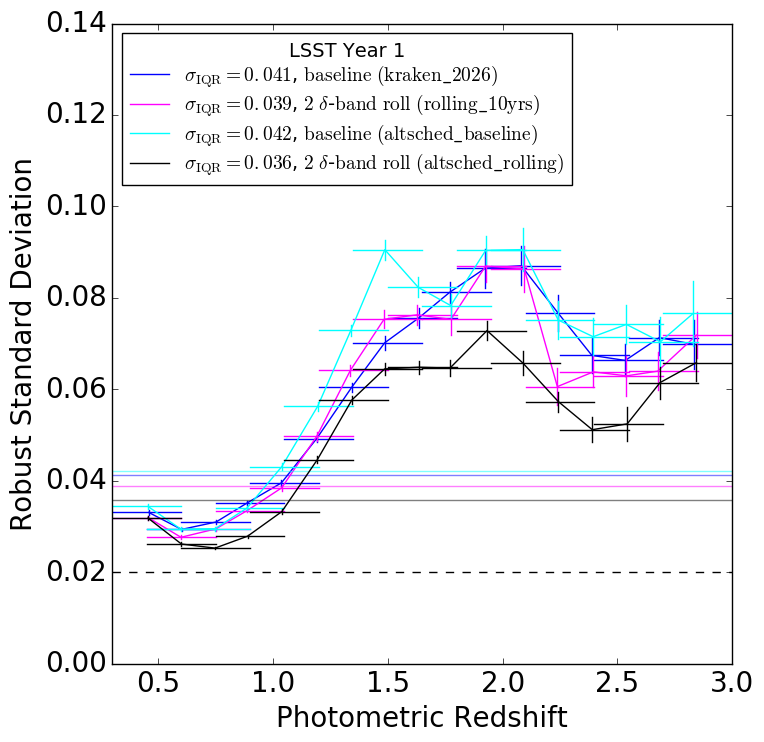
\includegraphics[width=6cm,trim={0cm 0cm 0cm 0cm},clip]{figures/ALTyear1_IQRs.png}
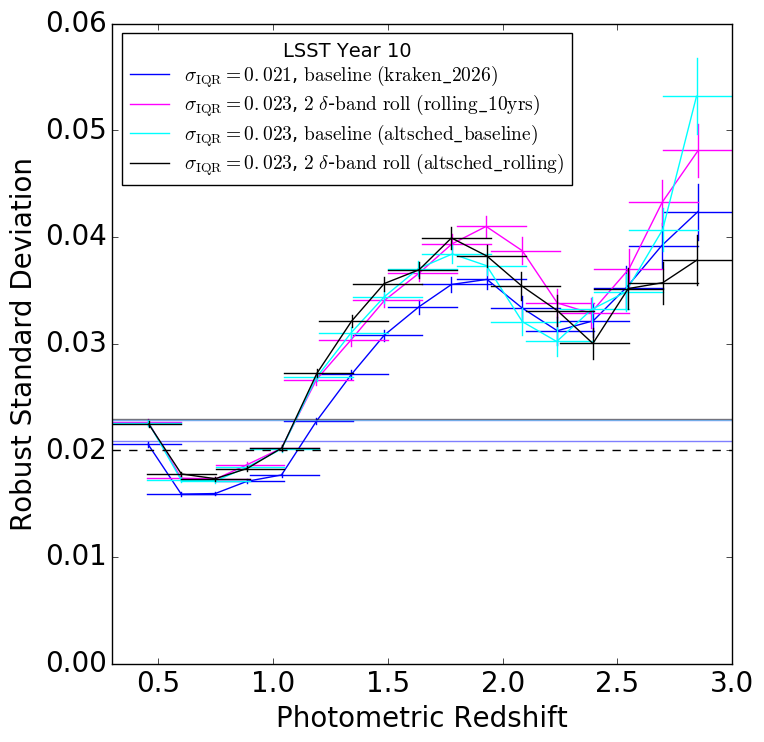
\includegraphics[width=6cm,trim={0cm 0cm 0cm 0cm},clip]{figures/ALTyear10_IQRs.png}
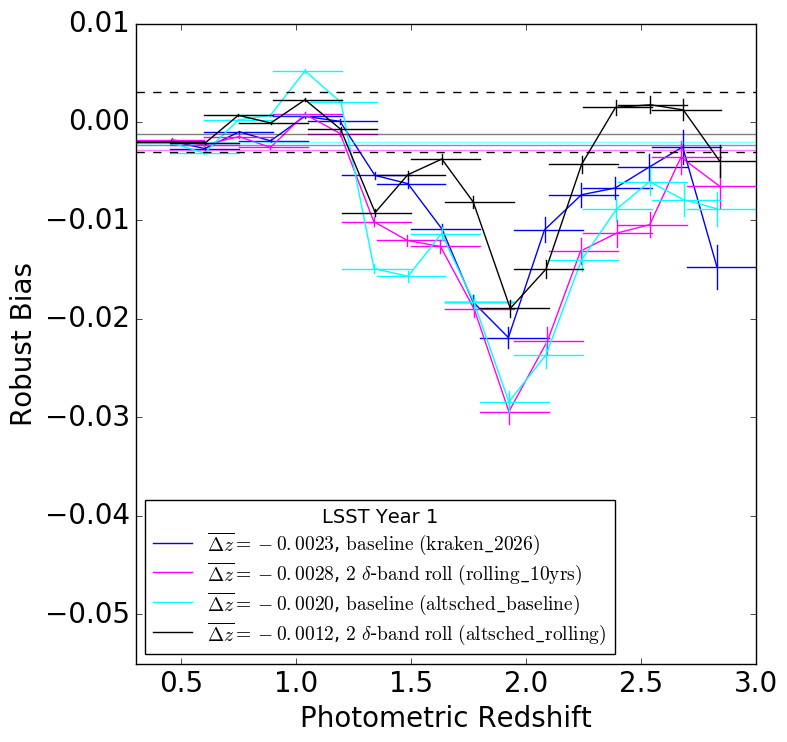
\includegraphics[width=6cm,trim={0cm 0cm 0cm 0cm},clip]{figures/ALTyear1_bias.png}
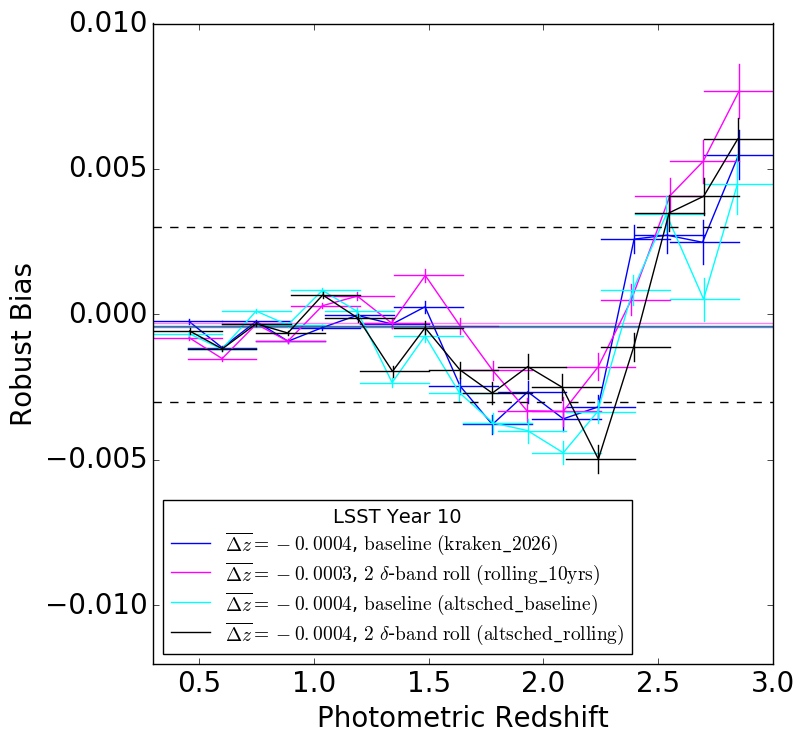
\includegraphics[width=6cm,trim={0cm 0cm 0cm 0cm},clip]{figures/ALTyear10_bias.png}
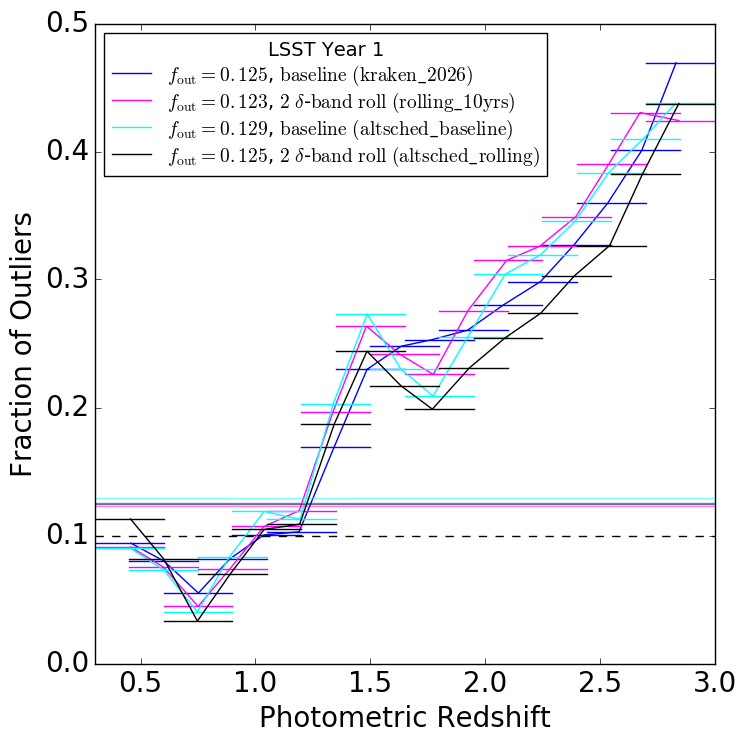
\includegraphics[width=6cm,trim={0cm 0cm 0cm 0cm},clip]{figures/ALTyear1_fout.png}
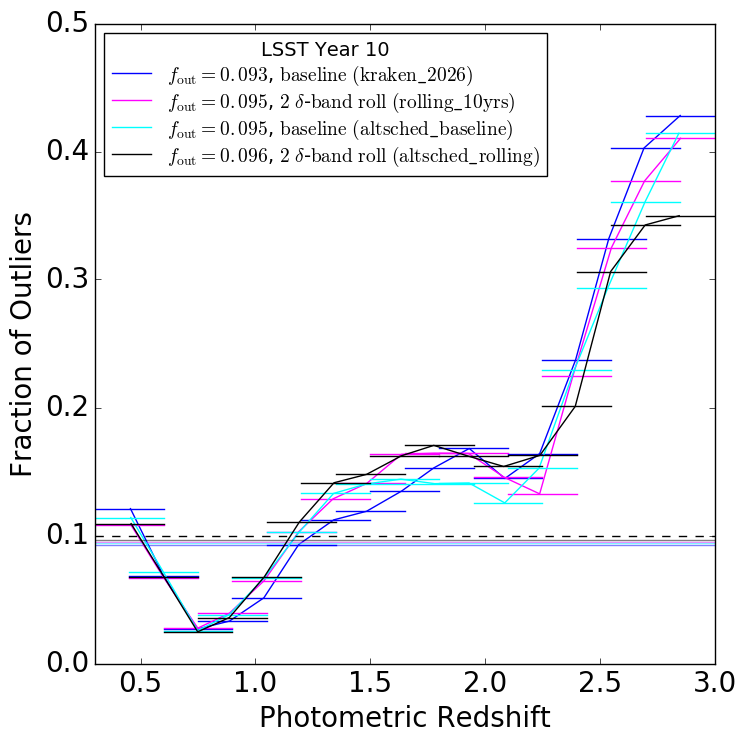
\includegraphics[width=6cm,trim={0cm 0cm 0cm 0cm},clip]{figures/ALTyear10_fout.png}
\caption{Statistical measures of robust standard deviation (from the IQR; top), robust bias (middle), and fraction of outliers (bottom) as a function of photo-$z$, at years $1$ (left column) and $10$ (right column). Note that the $y$-axes are not matched between columns. Results are presented for the {\tt OpSim} baseline ({\tt kraken\_2026}; blue) and rolling cadence ({\tt rolling\_10yrs}; magenta), and the {\tt ALTSched} baseline ({\tt altsched\_baseline}; cyan) and rolling cadence ({\tt altsched\_rolling}; black). Horizontal dashed line represents the LSST Science Requirement Document's target for a photo-$z$ bin of $0.3 \leq z_{\rm phot} \leq 3.0$., and horizontal colored bars represent the statistical for a photo-$z$ bin of $0.3 \leq z_{\rm phot} \leq 3.0$. \label{fig:stats_altsched}}
\end{center}
\end{figure}

\begin{figure}
\begin{center}
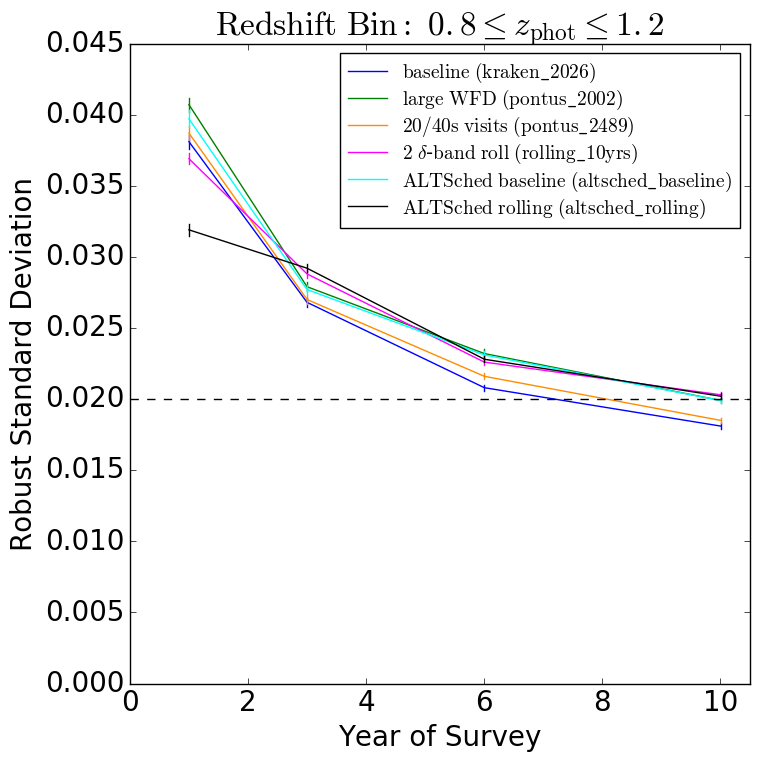
\includegraphics[width=6cm,trim={0cm 0cm 0cm 0cm},clip]{figures/zbin1_IQRs.png}
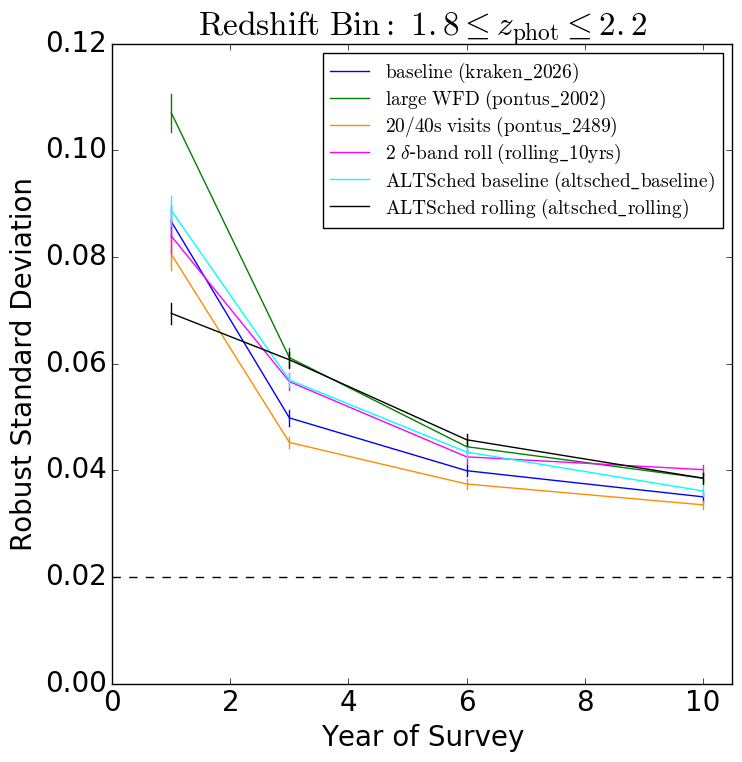
\includegraphics[width=6cm,trim={0cm 0cm 0cm 0cm},clip]{figures/zbin2_IQRs.png}
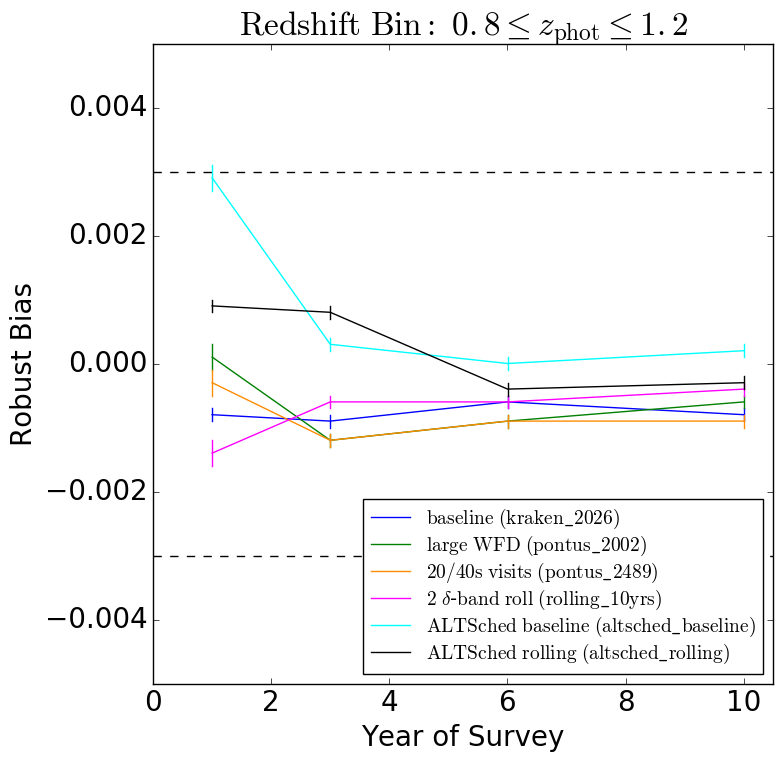
\includegraphics[width=6cm,trim={0cm 0cm 0cm 0cm},clip]{figures/zbin1_bias.png}
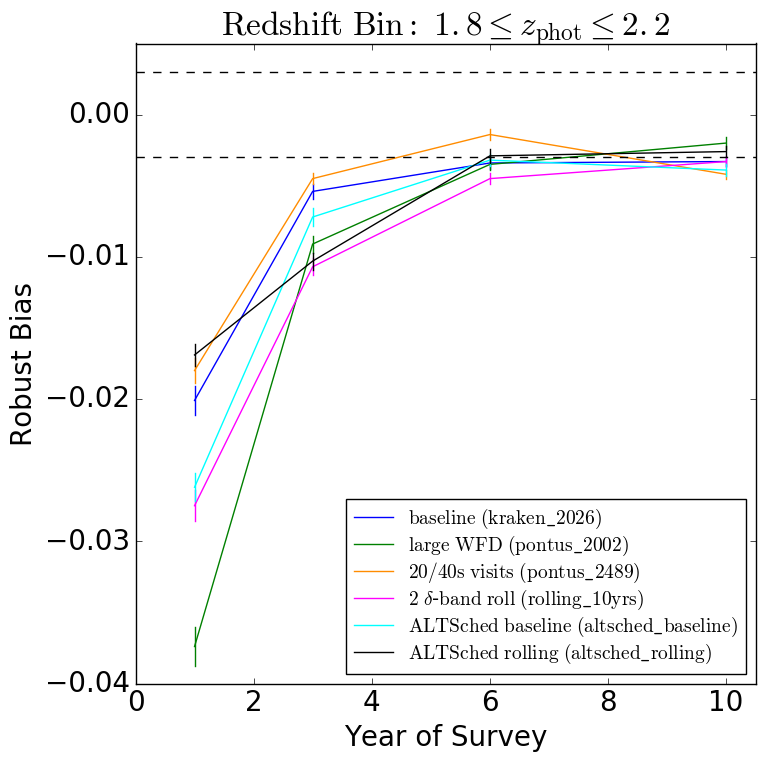
\includegraphics[width=6cm,trim={0cm 0cm 0cm 0cm},clip]{figures/zbin2_bias.png}
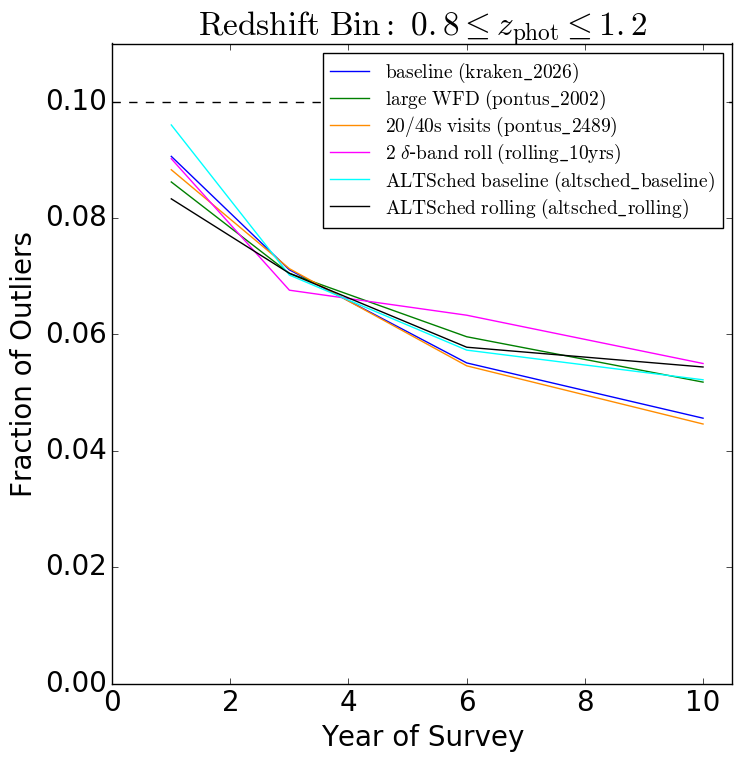
\includegraphics[width=6cm,trim={0cm 0cm 0cm 0cm},clip]{figures/zbin1_fout.png}
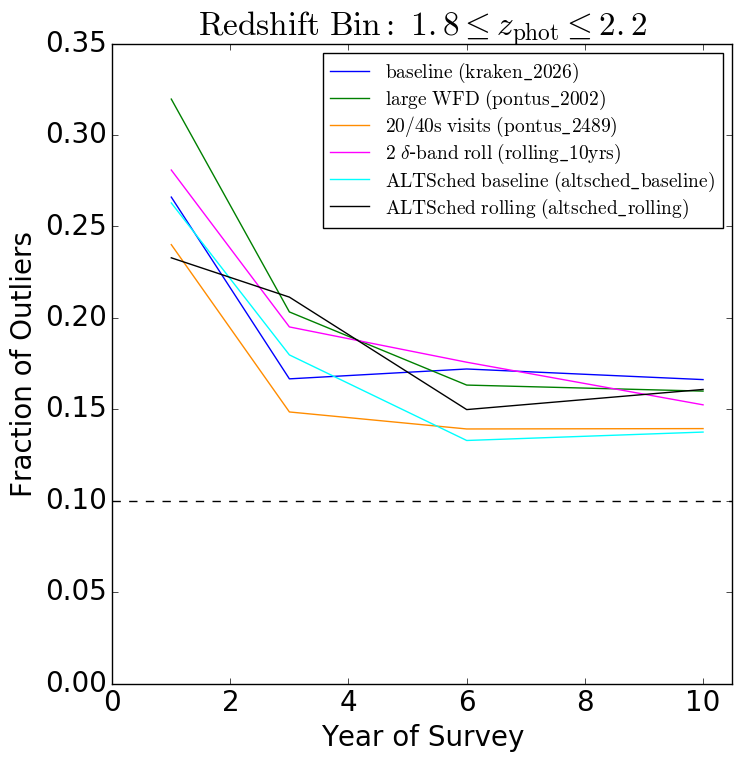
\includegraphics[width=6cm,trim={0cm 0cm 0cm 0cm},clip]{figures/zbin2_fout.png}
\caption{Statistical measures of robust standard deviation (from the IQR; top), robust bias (middle), and fraction of outliers (bottom) as a function of the LSST survey year, for bins of photometric redshift $0.8 \leq z_{\rm phot} \leq 1.2$ (left column) and  $1.8 \leq z_{\rm phot} \leq 2.2$ (right column). Note that the $y$-axes are not matched between columns. Results are presented for the baseline ({\tt kraken\_2026}; blue), large WFD area with declinations including  $-78<\delta<+18$ degrees ({\tt pontus\_2002}; green), the ``many visits" strategy with 40/20 second exposures in $u$/$grizy$ filters ({\tt pontus\_2489}; orange), a rolling cadence with two declination bands ({\tt rolling\_10yrs}; magenta), and the {\tt ALTSched} results for a baseline (cyan) and rolling (black) cadence. Horizontal dashed line represents the LSST Science Requirement Document's target for a photo-$z$ bin of $0.3 \leq z_{\rm phot} \leq 3.0$. \label{fig:evol}}
\end{center}
\end{figure}

\begin{table}\label{tab:zbins}
\caption{Relative Robust Standard Deviation of the Simulated Photometric Redshifts}
\begin{center}
\begin{tabular}{|l|cc|cc|cc|cc|}
\hline
{\tt OpSim}/{\tt ALTSched} Run & \multicolumn{2}{|c|}{Year 1} & \multicolumn{2}{|c|}{Year 3} & \multicolumn{2}{|c|}{Year 6} & \multicolumn{2}{|c|}{Year 10} \\ 
\multicolumn{1}{|r|}{$z_{\rm phot}$ Bin:} & 0.3--1.5 & 1.5--3.0 & 0.3--1.5 & 1.5--3.0 & 0.3--1.5 & 1.5--3.0 & 0.3--1.5 & 1.5--3.0 \\
\hline
baseline (kraken\_2026)                 & 1.95 & 4.07 & 1.42 & 2.58 & 1.15 & 2.05 & {\bf 1.00} & 1.83 \\ 
large WFD (pontus\_2002)                & 2.04 & 4.83 & 1.54 & 3.13 & 1.28 & 2.37 & 1.10 & 1.98 \\
many visits (pontus\_2489)              & 1.96 & 4.03 & 1.42 & 2.48 & 1.17 & 2.03 & 1.02 & 1.73 \\
$2$ $\delta$-band roll (rolling\_10yrs) & 1.87 & 3.92 & 1.53 & 3.04 & 1.24 & 2.29 & 1.10 & 1.98 \\
{\tt ALTSched} baseline                       & 1.98 & 4.35 & 1.52 & 2.89 & 1.25 & 2.28 & 1.11 & 1.95 \\
{\tt ALTSched} rolling                        & 1.69 & 3.38 & 1.55 & 3.08 & 1.26 & 2.35 & 1.11 & 1.93 \\
\hline
\end{tabular}
\end{center}
\end{table}


% % % % % % % % % % % % % % % % % % % % % % % % % % % % %
\subsection{Summary of Key Results} \label{ssec:pz_execsum}

\noindent
1. Most of the {\tt OpSim} and {\tt ALTSched} observing strategies result in a similar evolution of the median photometric depth in each filter, except: (a) when the WFD area is extended to $24,700$ square degrees (degraded photometric depth); (b) when 20/40 second visits are used for $grizy$/$u$ filters (improved photometric depth in $u$-band); or (c) when a rolling cadence is adopted (improved photometric depth of observed area in year 1). Photo-$z$ results are only simulated for these strategies that deliver a different photometric depth compared to the baseline cadence.

\medskip \noindent
2. The observing strategy in which 20/40 second visits are used for $grizy$/$u$ is the only one which exhibits improvements to the photo-$z$ quality over the baseline cadence option.

\medskip \noindent
3. The {\tt OpSim} and {\tt ALTSched} simulations offer essentially equivalent photo-$z$ results, with the exception that the {\tt ALTSched} rolling cadence delivers a significant improvement in year 1 only. We attribute the latter to the fact that the {\tt ALTSched} rolling cadence does not allocate any visits to the deprioritized declination band, whereas {\tt OpSim}'s rolling cadence allows it $25\%$ of the baseline number of visits.

